\chapter {Forecast}

The forecasting has been implemented in three differents ways: LSTM, SARIMA, MLP.
We have chosen to work on a smaller subset of data to speed up the comparison phase between the models.
The dataset used in forecasting evaluation is composed in fact by the players present in all three seasons and numer of matches played greater then 100.
The result is a 25 players dataset. 
Each player's fantavotes has been divided into train set and test set (70\% - 30\%).
The performances are compared in table \ref{table:RMSE} using RMSE as common metric.

\section{SARIMA}

Regarding SARIMA, \textit{auto-arima} function has been used to find the best parameters for the ARIMA model.


\begin{figure}[H]
  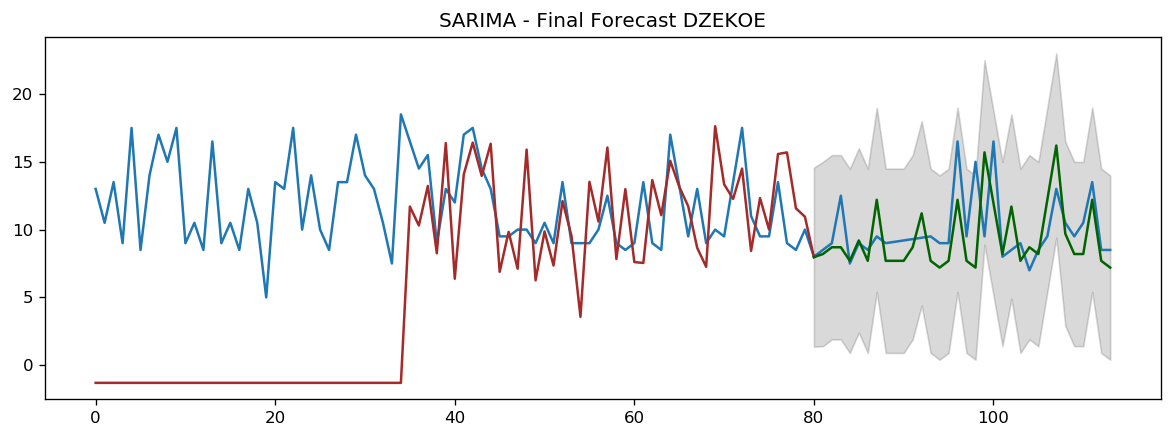
\includegraphics[scale=0.5]{images/dzeko_sarima_fantavoti.png}
   \caption{\textit{SARIMA forecast on ''Edin Dzeko''.}}
  \label{fig:sarima}
\end{figure}

\section{MLP}
The MLP model architecture includes 1 input layer with 12 nodes, 1 hidden layer with 38 nodes and 1 output layers with 1 node. The activation function is \textit{relu}.
The network has been trained with Adam optimizer and 150 epochs.

\begin{figure}[H]
  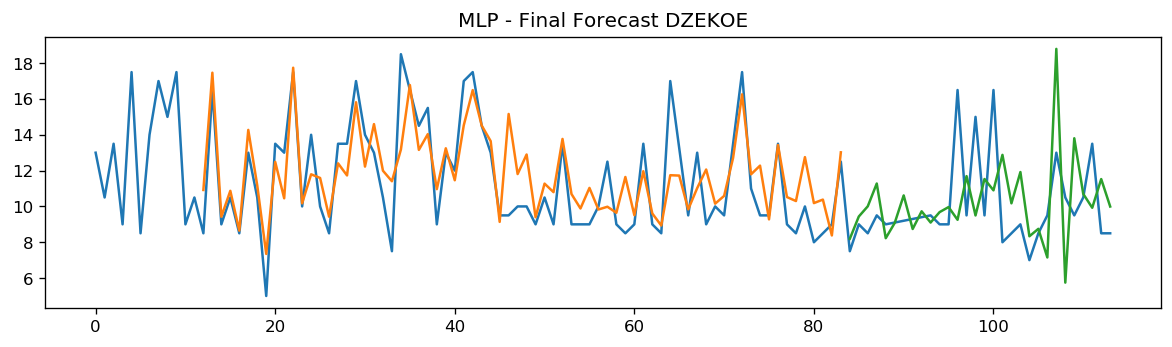
\includegraphics[scale=0.5]{images/dzeko_mlp_fantavoti.png}
   \caption{\textit{MLP forecast on ''Edin Dzeko''.}}
  \label{fig:sarima}
\end{figure}

\section{LSTM}

\begin{table}
 \begin{tabular}{|c|c|c|c|} 
 \hline
 Filling method & LSTM & SARIMA & MLP \\
 \hline \hline
 Linear interpolation & 0 & 1.97 & 2.21 \\
 Placeholder & 0 & 4.73 & 4.30  \\
 \hline
 \end{tabular}
 \caption{\textit{Comparison between different models and filling methods using RMSE.}}
 \label{table:RMSE}
\end{table}



The final model used for forecasting is defined as a linear combination of MLP and SARIMA, as follow:
\\
\begin{center}
  $\alpha * MLP + (1 - \alpha) * SARIMA$
\end{center}
where $\alpha$ is the parameter value that minimizes the RMSE (Root Mean Square Error).


